
\documentclass[12pt,a4paper]{article}

% =========================================================
% PACKAGES
% =========================================================
\usepackage[a4paper,margin=1in]{geometry}
\usepackage[T1]{fontenc}
\usepackage{lmodern}
\usepackage{microtype}
\usepackage{graphicx}
\usepackage{float}
\usepackage{array}
\usepackage{booktabs}
\usepackage{tabularx}
\usepackage{enumitem}
\usepackage{xcolor}
\usepackage{hyperref}
\usepackage{listings}
\usepackage{ragged2e}
\usepackage{caption}
\usepackage{makecell}


% =========================================================
% GENERAL FORMATTING
% =========================================================
\setlength{\parindent}{0pt}
\setlength{\parskip}{0.65em}
\setlist[itemize]{leftmargin=1.6em,itemsep=0.25em,topsep=0.3em}
\setlist[enumerate]{leftmargin=1.8em,itemsep=0.25em,topsep=0.3em}
\renewcommand{\arraystretch}{1.2}
\emergencystretch=2em

\definecolor{TitleBlue}{RGB}{31,78,121}
\definecolor{LightBlue}{RGB}{221,235,247}
\definecolor{LightGray}{RGB}{245,245,245}
\definecolor{CodeBlue}{RGB}{0,74,173}
\definecolor{CodeGreen}{RGB}{0,115,70}

\hypersetup{
    colorlinks=true,
    linkcolor=TitleBlue,
    urlcolor=TitleBlue,
    citecolor=TitleBlue,
    pdftitle={Design Patterns and Design Principles Report},
    pdfauthor={Najib Attar}
}

\newcolumntype{Y}{>{\RaggedRight\arraybackslash}X}
\newcolumntype{L}[1]{>{\RaggedRight\arraybackslash}p{#1}}

% =========================================================
% CODE STYLE
% =========================================================
\lstset{
    basicstyle=\ttfamily\small,
    keywordstyle=\color{CodeBlue}\bfseries,
    commentstyle=\color{CodeGreen},
    stringstyle=\color{purple},
    backgroundcolor=\color{LightGray},
    frame=single,
    rulecolor=\color{gray!40},
    breaklines=true,
    columns=fullflexible,
    showstringspaces=false,
    aboveskip=0.7em,
    belowskip=0.7em
}

% =========================================================
% TITLE
% =========================================================
\title{
    \textbf{\color{TitleBlue}Design Patterns and Design Principles Report}\\[0.4em]
    \large Resource Allocation System
}
\author{Najib Attar}
\date{}

\begin{document}

\maketitle
\tableofcontents
\newpage

% =========================================================
\section{Introduction}
% =========================================================

This report explains the object-oriented design of the Resource Allocation
System. The project contains a C++ backend and a Flask-based web dashboard.
The backend manages users, spaces, requests, validation rules, allocation
strategies, exam room sharing, committee meeting availability, data loading,
result exporting, and structured summaries.

The aim of the report is not to claim that every known design pattern was
used. Instead, it identifies the patterns and principles that solve real
problems in the system and explains why some other patterns were intentionally
not introduced.

For each major pattern, the report answers four questions:

\begin{enumerate}
    \item What does the pattern mean?
    \item Where is it used in the project?
    \item What problem does it solve?
    \item What benefit does it provide?
\end{enumerate}

The project currently applies several GRASP responsibilities, selected GoF
patterns, and general object-oriented design principles. The strongest examples
are Strategy, factory-style creation, Facade, Adapter, Polymorphism,
Pure Fabrication, Low Coupling, and Protected Variation.

% =========================================================
\section{Project Design Overview}
% =========================================================

The project is divided into the following main areas:

\begin{itemize}
    \item \path{src/models/}: domain classes such as \texttt{User},
    \texttt{Request}, \texttt{Space}, \texttt{Allocation}, and
    \texttt{TimeSlot}, together with their subclasses.

    \item \path{src/rules/}: independent validation rules such as
    \texttt{CapacityRule}, \texttt{FeatureRule}, \texttt{UserRoleRule},
    \texttt{RequestTypeRule}, and \texttt{ParticipantAvailabilityRule}.

    \item \path{src/strategies/}: allocation algorithms implementing
    \texttt{IAllocationStrategy}.

    \item \path{src/services/}: application services such as
    \texttt{AllocationService}, \texttt{ResourceAllocationSession},
    \texttt{UserAvailabilityService}, and
    \texttt{MeetingTimeSuggestionService}.

    \item \path{src/data/}: data loading and exporting components such as
    \texttt{DataLoader}, \texttt{DataController},
    \texttt{AllocationWriter}, \texttt{RequestResultWriter}, and
    \texttt{SummaryWriter}.

    \item \path{web/}: Flask routes, templates, form handling, and
    \texttt{BackendResultAdapter}.
\end{itemize}

The main architectural separation is:

\begin{center}
\textbf{Flask View and Input Layer}
$\longrightarrow$
\textbf{Backend Result Adapter}
$\longrightarrow$
\textbf{C++ Application and Domain Layers}
\end{center}

The C++ backend owns the allocation and validation behavior. Flask receives
input and presents backend-generated results. Therefore, the backend can still
compile and run without the web dashboard.

The following sections include focused diagrams for the main structural
patterns. Separate diagrams are used because a single complete class diagram
would be too dense to read clearly on an A4 page.

% =========================================================
\section{Main GoF Patterns Applied}
% =========================================================

This section explains the main GoF patterns that are actually implemented in
the project.

% ---------------------------------------------------------
\subsection{Strategy Pattern}
% ---------------------------------------------------------

\textbf{Meaning.}
The Strategy pattern defines a common interface for a family of algorithms.
The client uses the interface without depending directly on one specific
algorithm.

\textbf{Where it is used.}

\begin{itemize}
    \item \texttt{IAllocationStrategy}
    \item \texttt{GreedyAllocationStrategy}
    \item \texttt{PriorityAllocationStrategy}
    \item \texttt{MultiRoomExamGreedyStrategy}
    \item \texttt{MultiRoomExamBestFitStrategy}
    \item \texttt{SharedRoomExamBestFitStrategy}
    \item \texttt{AllocationService}
    \item \texttt{AllocationStrategyFactory}
\end{itemize}

As shown in Figure~\ref{fig:strategy-pattern}, the session obtains the
configured allocation strategy through \texttt{AllocationStrategyFactory}.
\texttt{AllocationService} then delegates request processing to the common
\texttt{IAllocationStrategy} interface.

\begin{figure}[H]
    \centering
    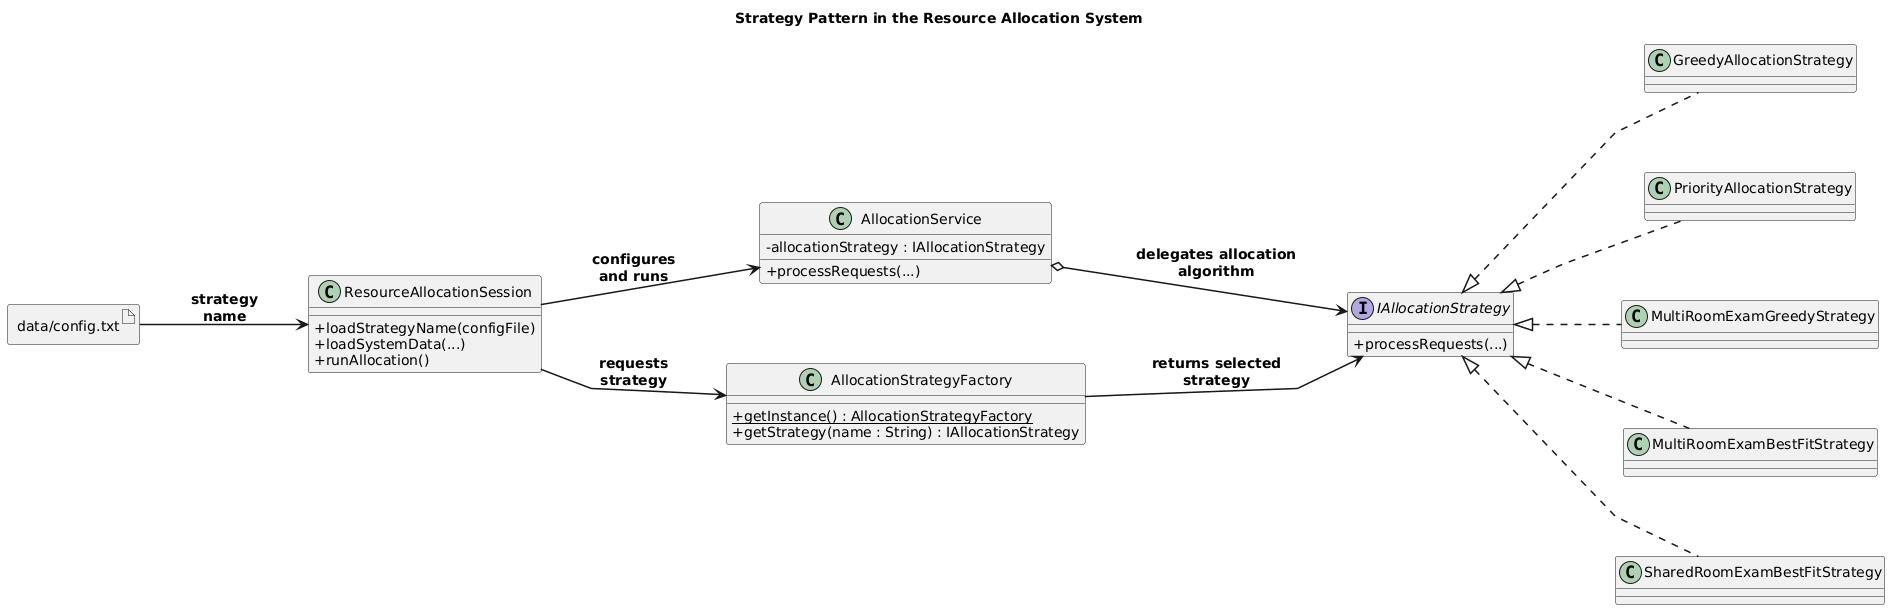
\includegraphics[width=1.1\textwidth]{diagrams/strategy-pattern.pdf}
    \caption{Strategy pattern and configuration-based algorithm selection.}
    \label{fig:strategy-pattern}
\end{figure}

\textbf{Small project example.}

\begin{lstlisting}[language=C++]
const IAllocationStrategy* strategy =
    AllocationStrategyFactory::getInstance()
        .getStrategy(strategyName);

strategy->processRequests(
    requests,
    spaces,
    allocations,
    ruleEngineFacade
);
\end{lstlisting}

\textbf{Why it was used.}
The allocation algorithm is a major variation point. The system may process
requests using CSV order, priority order, multi-room best fit, or shared-room
best fit.

\textbf{Problem solved.}
Without Strategy, \texttt{AllocationService} would require many conditional
statements for every allocation algorithm.

\textbf{Main benefits.}

\begin{itemize}
    \item New allocation algorithms can implement the same interface.
    \item Existing service logic does not need to be rewritten.
    \item The selected strategy can be changed through configuration.
    \item The design supports Low Coupling and the Open/Closed Principle.
\end{itemize}

% ---------------------------------------------------------
\subsection{Factory-Style Object Creation}
% ---------------------------------------------------------

\textbf{Meaning.}
A factory centralizes the decision about which concrete subclass should be
created.

The project mainly uses static or simple factories. Therefore, it is more
accurate to call this \textbf{factory-style creation} rather than strict GoF
Factory Method inheritance.

\subsubsection*{UserFactory}

\textbf{Input:} user ID, name, role name, and profile information.

\textbf{Creates:}

\begin{itemize}
    \item \texttt{Student}
    \item \texttt{TeachingAssistant}
    \item \texttt{Staff}
    \item \texttt{Instructor}
    \item \texttt{Administrator}
\end{itemize}

\subsubsection*{RequestFactory}

\textbf{Input:} request type, requester, requested space, participant count,
metadata, and time data.

\textbf{Creates:}

\begin{itemize}
    \item \texttt{OneTimeRequest}
    \item \texttt{RecurringRequest}
    \item \texttt{ExamRequest}
    \item \texttt{CommitteeMeetingRequest}
    \item \texttt{InvalidRequest}
\end{itemize}

Malformed or unsupported request input can be represented safely as an
\texttt{InvalidRequest} instead of causing a crash.

\subsubsection*{SpaceFactory}

\textbf{Input:} space type, ID, name, capacity, feature flags, availability,
and building.

\textbf{Creates:}

\begin{itemize}
    \item \texttt{Classroom}
    \item \texttt{Laboratory}
    \item \texttt{MeetingRoom}
\end{itemize}

Before Iteration 40, \texttt{DataLoader} directly selected and constructed the
concrete space classes. After introducing \texttt{SpaceFactory},
\texttt{DataLoader} only parses and validates CSV data.

\subsubsection*{AllocationStrategyFactory}

\textbf{Input:} strategy name from \path{data/config.txt}.

\textbf{Returns:} an implementation of \texttt{IAllocationStrategy}.

Unknown or empty strategy names are handled using the existing safe fallback
behavior.

Figure~\ref{fig:factory-polymorphism} shows how
\texttt{DataLoader} remains responsible for reading and validating external
data, while the factories decide which concrete polymorphic objects should be
created.

\begin{figure}[H]
    \centering
    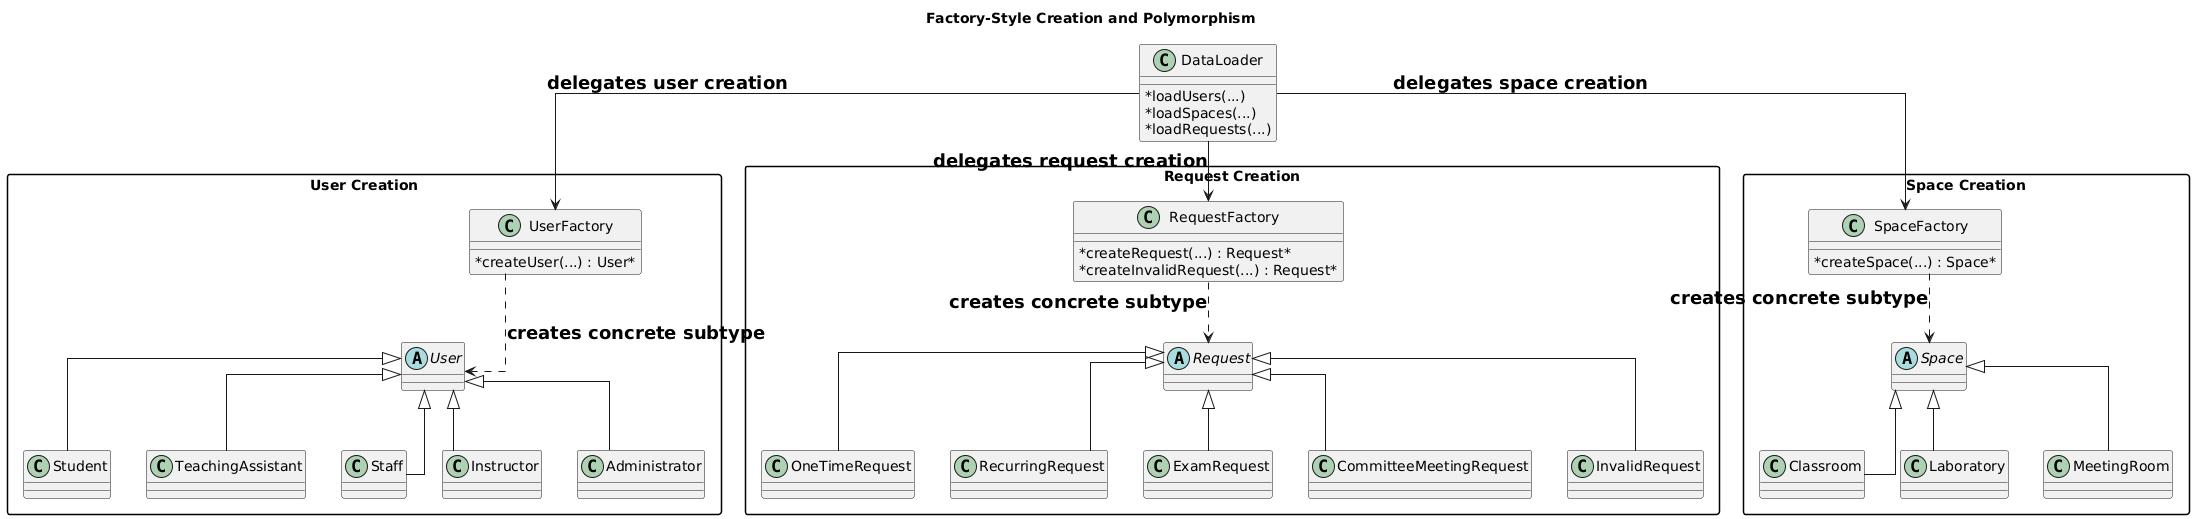
\includegraphics[width=1.1\textwidth]{diagrams/factory-polymorphism.pdf}
    \caption{Factory-style creation for users, requests, and spaces.}
    \label{fig:factory-polymorphism}
\end{figure}

\textbf{Small project example.}

\begin{lstlisting}[language=C++]
Space* space = SpaceFactory::createSpace(
    id,
    name,
    type,
    capacity,
    hasProjector,
    hasWhiteboard,
    hasComputers,
    isAvailable,
    building
);
\end{lstlisting}

\textbf{Problem solved.}
CSV parsing classes no longer need to contain all concrete object-construction
decisions.

\textbf{Main benefits.}

\begin{itemize}
    \item Creation logic is centralized.
    \item Loaders and services have fewer concrete dependencies.
    \item Unsupported type values are handled consistently.
    \item Adding a new concrete subtype has a clear extension point.
\end{itemize}

% ---------------------------------------------------------
\subsection{Facade Pattern}
% ---------------------------------------------------------

\textbf{Meaning.}
A Facade provides a simple entry point to a more complex subsystem.

Two different facades are used in the project.

\subsubsection*{ResourceAllocationSession}

\texttt{ResourceAllocationSession} is the application-level backend facade.
It coordinates:

\begin{itemize}
    \item strategy configuration loading,
    \item system data loading,
    \item allocation execution,
    \item result exporting,
    \item structured summary exporting, and
    \item cleanup.
\end{itemize}

\begin{lstlisting}[language=C++]
ResourceAllocationSession session;

session.loadStrategyName("data/config.txt");
session.loadSystemData(...);
session.runAllocation();
session.exportResults(...);
session.cleanup();
\end{lstlisting}

This keeps \texttt{main.cpp} small and prepares the backend to be used by a
future CLI, REST interface, desktop application, or alternative frontend.

\subsubsection*{RuleEngineFacade}

\texttt{RuleEngineFacade} is a smaller facade focused only on rule evaluation.
It hides the internal rule pipeline from allocation strategies.

The two facade levels are shown in
Figure~\ref{fig:facade-pattern}. \texttt{ResourceAllocationSession}
simplifies the complete backend workflow, while
\texttt{RuleEngineFacade} simplifies access to the rule subsystem.

\begin{figure}[H]
    \centering
    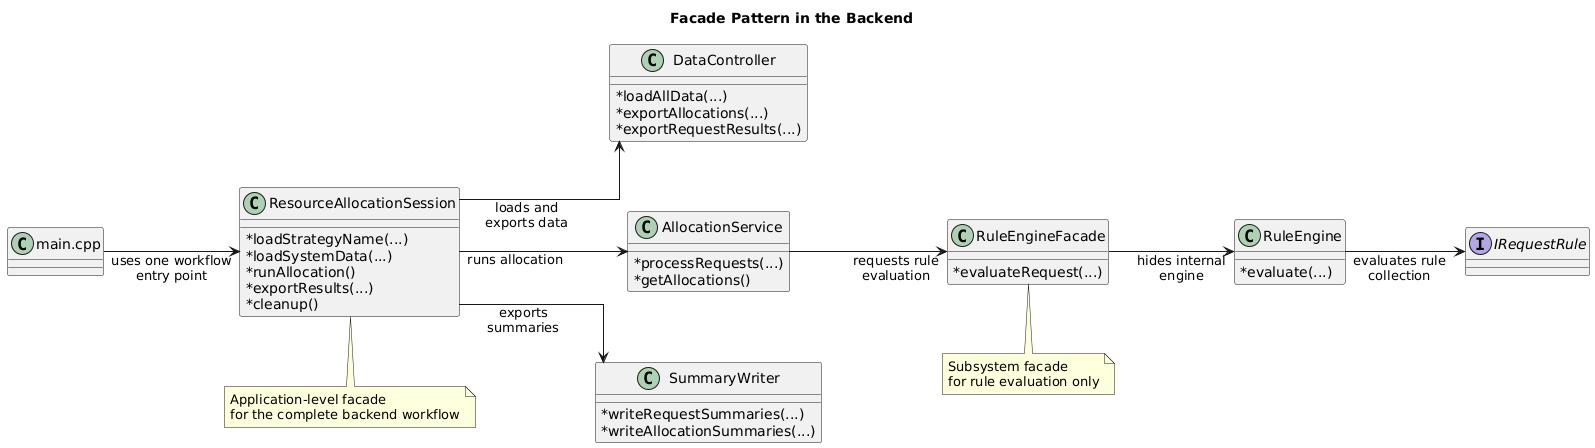
\includegraphics[width=1.1\textwidth]{diagrams/facade-pattern.pdf}
    \caption{Application-level and subsystem-level facades.}
    \label{fig:facade-pattern}
\end{figure}

\textbf{Difference between the two facades.}

\begin{table}[H]
    \centering
    \caption{Responsibilities of the two facade classes.}
    \begin{tabularx}{\textwidth}{L{4.2cm}YY}
        \toprule
        \textbf{Facade} & \textbf{Scope} & \textbf{Main Responsibility} \\
        \midrule
\makecell[l]{ResourceAllocation\\Session}        & Full backend workflow
        & Load data, select strategy, run allocation, export results, and clean up. \\

        \texttt{RuleEngineFacade}
        & Rule subsystem
        & Give strategies one simple method for evaluating request rules. \\
        \bottomrule
    \end{tabularx}
\end{table}

% ---------------------------------------------------------
\subsection{Adapter Pattern}
% ---------------------------------------------------------

\textbf{Meaning.}
An Adapter converts an existing interface or data representation into a form
that a client can use more easily.

\textbf{Where it is used.}

\begin{itemize}
    \item \path{web/backend_result_adapter.py}
    \item \texttt{BackendResultAdapter}
    \item Flask routes in \path{web/app.py}
\end{itemize}

As shown in Figure~\ref{fig:adapter-pattern}, Flask routes no longer need to
understand and combine every backend result file directly. They request
UI-ready structures from \texttt{BackendResultAdapter}.

\begin{figure}[H]
    \centering
    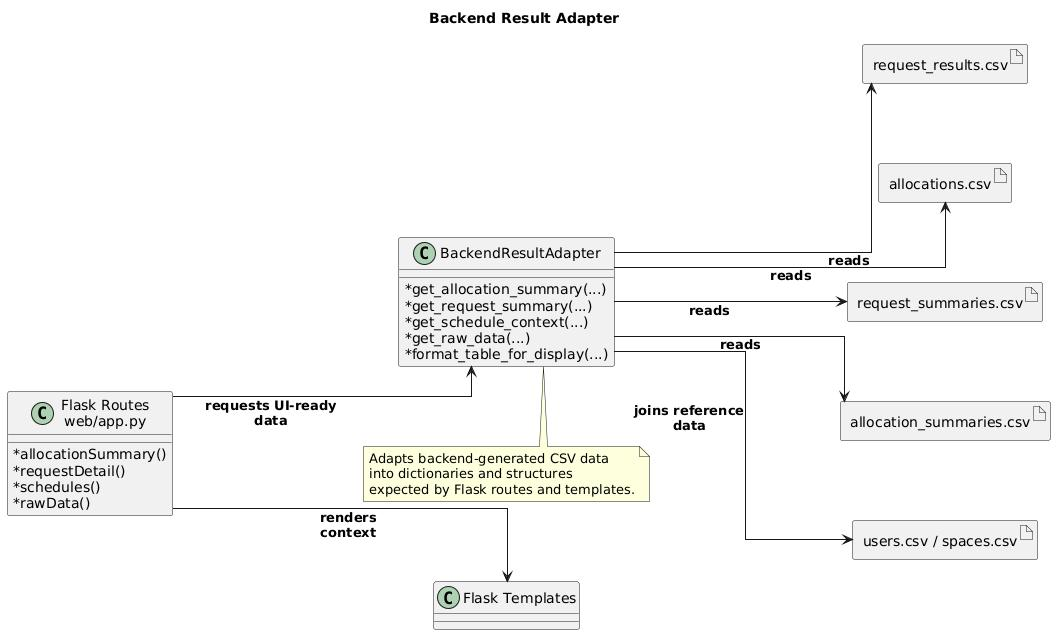
\includegraphics[width=1.1\textwidth]{diagrams/adapter-pattern.pdf}
    \caption{Adapter between Flask routes and backend-generated result files.}
    \label{fig:adapter-pattern}
\end{figure}

\textbf{Small project example.}

\begin{lstlisting}[language=Python]
adapter = BackendResultAdapter(DATA_DIR)

summary = adapter.get_allocation_summary(strategy)
schedule = adapter.get_schedule_context("user", user_id)
request = adapter.get_request_summary(request_id, strategy)
\end{lstlisting}

\textbf{Why it was used.}
The Flask routes previously contained repeated logic for reading CSV files,
joining results, building schedules, handling missing requests, and formatting
summary information.

\textbf{Problem solved.}
The adapter hides backend output details from Flask route functions.

\textbf{Main benefits.}

\begin{itemize}
    \item Flask routes remain focused on HTTP and UI flow.
    \item Result-reading logic is centralized.
    \item Changes to output interpretation affect fewer route functions.
    \item Schedule reconstruction and external allocation handling are consistent.
    \item Model--View separation is improved.
\end{itemize}

% ---------------------------------------------------------
\subsection{Singleton}
% ---------------------------------------------------------

\textbf{Status: Applied narrowly.}

\texttt{AllocationStrategyFactory} currently provides access through
\texttt{getInstance()}.

\begin{lstlisting}[language=C++]
AllocationStrategyFactory::getInstance()
    .getStrategy(strategyName);
\end{lstlisting}

The Singleton is intentionally not used throughout the project. Excessive
Singleton usage could introduce hidden global dependencies and make testing
more difficult.

The current strategy factory is mostly stateless, so a static factory could
also satisfy the present requirements. Therefore, the report treats Singleton
as a limited implementation choice rather than a pattern that should be
expanded to other classes.

% =========================================================
\section{GRASP Pattern Usage}
% =========================================================

GRASP patterns focus on assigning responsibilities to classes. The following
table provides a compact overview before the detailed explanations.

\begin{table}[H]
    \centering
    \small
    \caption{GRASP patterns used in the project.}
    \begin{tabularx}{\textwidth}{L{3.1cm}L{4.8cm}Y}
        \toprule
        \textbf{GRASP Pattern}
        & \textbf{Main Project Location}
        & \textbf{Responsibility / Benefit} \\
        \midrule

        Controller
        & \texttt{ResourceAllocationSession}; Flask routes
        & Coordinates system-level operations without performing all detailed work. \\

        Creator
        & User, request, space, and strategy factories
        & Centralizes polymorphic object creation from external type values. \\

        Information Expert
        & \texttt{TimeSlot}, \texttt{User}, \texttt{Request}, \texttt{Space}
        & Assigns behavior to the class that owns the required information. \\

        Low Coupling
        & Interfaces, facades, factories, adapter
        & Reduces the number of concrete dependencies between classes. \\

        High Cohesion
        & Focused rules, writers, services, and factories
        & Gives each class a small and understandable responsibility. \\

        Polymorphism
        & User, request, space, rule, and strategy hierarchies
        & Allows different types to be handled through common abstractions. \\

        Pure Fabrication
        & Controllers, services, writers, factories
        & Keeps technical responsibilities outside domain entities. \\

        Indirection
        & Facades, factories, and \texttt{BackendResultAdapter}
        & Adds stable boundaries between changing subsystems. \\

        Protected Variation
        & Strategy interface, factories, adapter
        & Protects stable code from expected areas of change. \\

        \bottomrule
    \end{tabularx}
\end{table}

% ---------------------------------------------------------
\subsection{Controller}
% ---------------------------------------------------------

\textbf{Primary controller:} \texttt{ResourceAllocationSession}.

It receives a system-level workflow request and coordinates other components.
It does not contain allocation algorithms or rule logic.

Flask routes also act as UI controllers because they receive HTTP requests,
validate form input, call application helpers, and select templates.

\texttt{DataController} is better described as a technical data coordinator
or Pure Fabrication rather than the main use-case controller.

% ---------------------------------------------------------
\subsection{Creator}
% ---------------------------------------------------------

The factories apply Creator by taking responsibility for constructing
polymorphic objects when the concrete type depends on external input.

For example:

\begin{center}
CSV role string
$\longrightarrow$
\texttt{UserFactory}
$\longrightarrow$
concrete \texttt{User} subclass
\end{center}

The same idea applies to requests, spaces, and allocation strategies.

% ---------------------------------------------------------
\subsection{Information Expert}
% ---------------------------------------------------------

Information Expert assigns behavior to the class that has the information
needed to perform it.

Examples include:

\begin{itemize}
    \item \texttt{TimeSlot::overlapsWith(...)} checks time overlap.
    \item \texttt{Space::hasFeature(...)} checks supported space features.
    \item User subclasses provide their own priority and permission behavior.
    \item \texttt{Request} maintains its status, rejection reason, and lifecycle history.
\end{itemize}

This avoids moving all behavior into one large manager or service class.

% ---------------------------------------------------------
\subsection{Low Coupling and High Cohesion}
% ---------------------------------------------------------

These two GRASP goals work together.

\textbf{Low Coupling} is supported by:

\begin{itemize}
    \item \texttt{IAllocationStrategy},
    \item \texttt{IRequestRule},
    \item factories,
    \item facades, and
    \item \texttt{BackendResultAdapter}.
\end{itemize}

\textbf{High Cohesion} is supported by focused classes:

\begin{itemize}
    \item \texttt{CapacityRule} checks capacity only.
    \item \texttt{FeatureRule} checks features only.
    \item \texttt{SpaceFactory} creates spaces only.
    \item \texttt{SummaryWriter} writes summary outputs only.
    \item \texttt{MeetingTimeSuggestionService} generates time suggestions.
\end{itemize}

The result is a system in which changes usually affect a limited set of files.

% ---------------------------------------------------------
\subsection{Polymorphism}
% ---------------------------------------------------------

Polymorphism is central to the design.

\begin{table}[H]
    \centering
    \small
    \caption{Main polymorphic hierarchies.}
    \begin{tabularx}{\textwidth}{L{3.4cm}Y}
        \toprule
        \textbf{Base Type} & \textbf{Concrete Types} \\
        \midrule

        \texttt{User}
        & \texttt{Student}, \texttt{TeachingAssistant}, \texttt{Staff},
        \texttt{Instructor}, \texttt{Administrator} \\

        \texttt{Request}
        & \texttt{OneTimeRequest}, \texttt{RecurringRequest},
        \texttt{ExamRequest}, \texttt{CommitteeMeetingRequest},
        \texttt{InvalidRequest} \\

        \texttt{Space}
        & \texttt{Classroom}, \texttt{Laboratory}, \texttt{MeetingRoom} \\

        \texttt{IAllocationStrategy}
        & Greedy, priority, multi-room, best-fit, and shared-room strategies \\

        \texttt{IRequestRule}
        & Capacity, feature, status, location, role, request type, and
        participant availability rules \\

        \bottomrule
    \end{tabularx}
\end{table}

Rule polymorphism is shown in Figure~\ref{fig:rule-polymorphism}.
\texttt{RuleEngine} evaluates rule objects through
\texttt{IRequestRule}, so it does not need a separate evaluation mechanism for
every concrete rule class.

\begin{figure}[H]
    \centering
    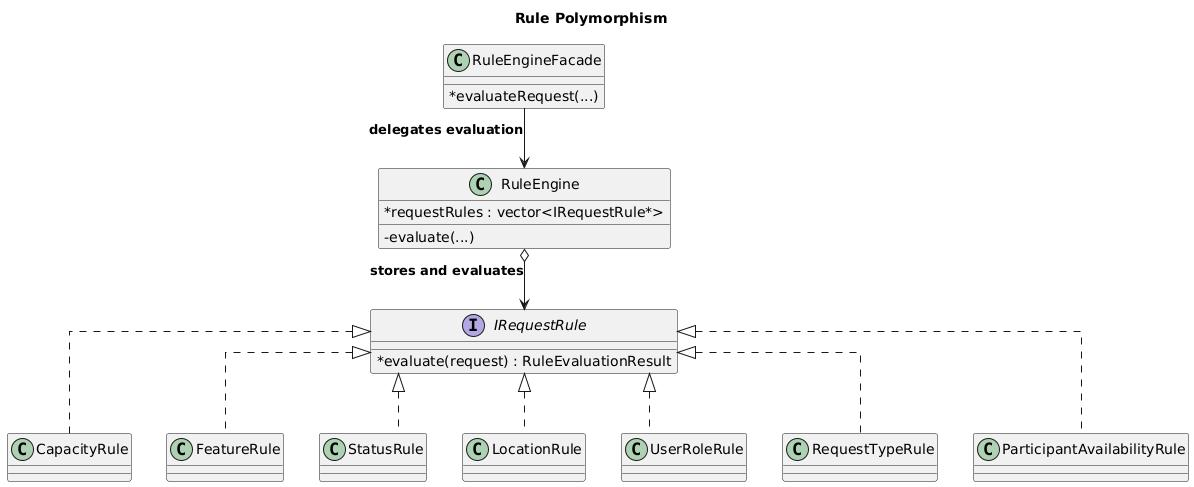
\includegraphics[width=1.1\textwidth]{diagrams/rule-polymorphism.pdf}
    \caption{Polymorphic request-rule evaluation.}
    \label{fig:rule-polymorphism}
\end{figure}

Polymorphism allows the rest of the system to use base pointers or interfaces
while concrete objects provide different behavior.

% ---------------------------------------------------------
\subsection{Pure Fabrication}
% ---------------------------------------------------------

Pure Fabrication introduces non-domain classes when they improve the design.

Examples include:

\begin{itemize}
    \item \texttt{DataController}
    \item \texttt{DataLoader}
    \item \texttt{ResourceAllocationSession}
    \item \texttt{SummaryWriter}
    \item \texttt{MeetingTimeSuggestionService}
    \item factory classes
    \item \texttt{BackendResultAdapter}
\end{itemize}

These are not physical university objects. They exist to keep technical
responsibilities out of domain classes such as \texttt{User},
\texttt{Request}, and \texttt{Space}.

% ---------------------------------------------------------
\subsection{Indirection and Protected Variation}
% ---------------------------------------------------------

\textbf{Indirection} introduces an intermediate object to reduce direct
dependency.

Examples:

\begin{itemize}
    \item \texttt{RuleEngineFacade} stands between strategies and the rule pipeline.
    \item \texttt{BackendResultAdapter} stands between Flask routes and result files.
    \item factories stand between CSV/configuration strings and concrete classes.
\end{itemize}

\textbf{Protected Variation} identifies expected areas of change and isolates
them behind stable boundaries.

\begin{table}[H]
    \centering
    \small
    \caption{Variation points protected by the design.}
    \begin{tabularx}{\textwidth}{L{4.3cm}Y}
        \toprule
        \textbf{Expected Variation} & \textbf{Protection Mechanism} \\
        \midrule

        Allocation algorithm
        & \texttt{IAllocationStrategy} and
        \texttt{AllocationStrategyFactory} \\

        User subtype
        & \texttt{User} hierarchy and \texttt{UserFactory} \\

        Request subtype
        & \texttt{Request} hierarchy and \texttt{RequestFactory} \\

        Space subtype
        & \texttt{Space} hierarchy and \texttt{SpaceFactory} \\

        Rule implementation
        & \texttt{IRequestRule} and \texttt{RuleEngineFacade} \\

        Flask result interpretation
        & \texttt{BackendResultAdapter} \\

        \bottomrule
    \end{tabularx}
\end{table}

% =========================================================
\section{Design Principles Usage}
% =========================================================

% ---------------------------------------------------------
\subsection{Model--View Separation}
% ---------------------------------------------------------

\textbf{Status: Mostly applied.}

The C++ backend contains domain logic, validation rules, strategies, factories,
services, participant availability, meeting suggestions, and result exporting.

Flask handles:

\begin{itemize}
    \item HTTP routes,
    \item forms,
    \item redirects,
    \item user-facing validation messages, and
    \item template rendering.
\end{itemize}

\texttt{BackendResultAdapter} improves the boundary by moving result-reading
and adaptation out of Flask route functions.

The separation is described as \emph{mostly applied} rather than completely
applied because Flask still understands some input CSV structures and writes
CSV-based request data.

% ---------------------------------------------------------
\subsection{Low Representation Gap}
% ---------------------------------------------------------

The software classes closely represent the real university allocation domain.

Examples include:

\begin{itemize}
    \item \texttt{User}
    \item \texttt{Space}
    \item \texttt{Request}
    \item \texttt{ExamRequest}
    \item \texttt{CommitteeMeetingRequest}
    \item \texttt{Allocation}
    \item \texttt{TimeSlot}
\end{itemize}

This makes the software easier to understand because its vocabulary is similar
to the real problem vocabulary.

% ---------------------------------------------------------
\subsection{Separation of Concerns}
% ---------------------------------------------------------

The project separates major concerns as follows:

\begin{table}[H]
    \centering
    \small
    \caption{Separation of concerns in the project.}
    \begin{tabularx}{\textwidth}{L{4.1cm}Y}
        \toprule
        \textbf{Concern} & \textbf{Responsible Area} \\
        \midrule

        Domain representation
        & \path{src/models/} \\

        Rule evaluation
        & \path{src/rules/} and \texttt{RuleEngineFacade} \\

        Allocation algorithms
        & \path{src/strategies/} \\

        Workflow coordination
        & \texttt{ResourceAllocationSession} and
        \texttt{AllocationService} \\

        Data loading and exporting
        & \path{src/data/} \\

        Backend-result adaptation
        & \texttt{BackendResultAdapter} \\

        User interface
        & Flask routes and templates \\

        \bottomrule
    \end{tabularx}
\end{table}

% ---------------------------------------------------------
\subsection{Design to Interface, Not Implementation}
% ---------------------------------------------------------

The system depends on abstractions where behavior is expected to vary.

\begin{lstlisting}[language=C++]
const IAllocationStrategy* strategy;
std::vector<IRequestRule*> requestRules;
\end{lstlisting}

\texttt{AllocationService} works with \texttt{IAllocationStrategy}, while the
rule engine works with \texttt{IRequestRule}.

This allows concrete implementations to vary without changing the main client
logic.

% ---------------------------------------------------------
\subsection{Open/Closed Principle}
% ---------------------------------------------------------

\textbf{Status: Partially applied.}

The system is open for extension through:

\begin{itemize}
    \item new allocation strategies,
    \item new rules,
    \item new user subclasses,
    \item new request subclasses, and
    \item new space subclasses.
\end{itemize}

For example, a new allocation algorithm can implement
\texttt{IAllocationStrategy} without rewriting \texttt{AllocationService}.

The principle is only partially applied because factories still require manual
registration of new type strings. This is acceptable for the current project
size and keeps object creation explicit.

% ---------------------------------------------------------
\subsection{Law of Demeter}
% ---------------------------------------------------------

\textbf{Status: Partially applied.}

Facades and adapters reduce the number of objects that each client must know.

For example:

\begin{itemize}
    \item \texttt{main.cpp} delegates backend workflow to
    \texttt{ResourceAllocationSession}.
    \item strategies delegate rule evaluation to \texttt{RuleEngineFacade}.
    \item Flask routes delegate result interpretation to
    \texttt{BackendResultAdapter}.
\end{itemize}

Some CSV field knowledge remains in the web input flow because requests are
currently submitted through CSV-based storage.

% ---------------------------------------------------------
\subsection{Find What Varies and Encapsulate It}
% ---------------------------------------------------------

The project identifies the following major variation points:

\begin{itemize}
    \item allocation algorithm,
    \item user type,
    \item request type,
    \item space type,
    \item rule implementation, and
    \item frontend interpretation of backend results.
\end{itemize}

These are encapsulated through strategies, factories, interfaces, facades, and
the adapter.

% ---------------------------------------------------------
\subsection{Favor Composition Over Inheritance}
% ---------------------------------------------------------

\textbf{Status: Applied with balance.}

Inheritance is used where the domain naturally contains ``is-a'' relationships,
such as:

\begin{itemize}
    \item \texttt{Student} is a \texttt{User},
    \item \texttt{ExamRequest} is a \texttt{Request}, and
    \item \texttt{Classroom} is a \texttt{Space}.
\end{itemize}

Composition is used to assemble application behavior.

Examples:

\begin{itemize}
    \item \texttt{ResourceAllocationSession} composes
    \texttt{DataController} and \texttt{AllocationService}.
    \item \texttt{AllocationService} collaborates with a strategy,
    \texttt{RuleEngineFacade}, and meeting suggestion service.
    \item \texttt{RuleEngine} contains a collection of rule objects.
\end{itemize}

The project therefore favors composition for coordination while retaining
inheritance where polymorphism is meaningful.

% ---------------------------------------------------------
\subsection{Low Coupling and High Cohesion}
% ---------------------------------------------------------

These principles are visible throughout the architecture.

\textbf{Low Coupling} means that changing one component should not require
changes throughout the entire project.

\textbf{High Cohesion} means that each component should have a clear,
focused responsibility.

Examples:

\begin{itemize}
    \item A new strategy mainly affects the strategy package and its factory.
    \item A new space type mainly affects the space hierarchy and
    \texttt{SpaceFactory}.
    \item Changing schedule display logic is concentrated in
    \texttt{BackendResultAdapter}.
    \item Each rule class checks one category of condition.
\end{itemize}

% =========================================================
\section{Patterns Intentionally Not Used}
% =========================================================

Not using a pattern can be the correct design decision. The following patterns
were considered but are not justified by the current requirements.

\begin{table}[H]
    \centering
    \small
    \caption{Patterns intentionally not used.}
    \begin{tabularx}{\textwidth}{L{3.4cm}Y}
        \toprule
        \textbf{Pattern} & \textbf{Reason It Is Not Used} \\
        \midrule

        Abstract Factory
        & The system does not need to create complete families of related
        products together. Separate factories are sufficient. \\

        Composite
        & Buildings, rooms, and organization units are not currently processed
        through uniform tree operations. \\

        Decorator
        & There is no requirement to add and remove object behavior dynamically
        through runtime wrappers. \\

        Bridge
        & The system does not yet have two independently varying hierarchies
        such as several report abstractions combined with several output
        implementations. \\

        Template Method
        & Strategy classes share some workflow ideas, but the duplication is
        not yet large enough to justify a rigid common algorithm skeleton. \\

        Observer
        & Request status changes do not currently have independent subscribers
        such as notification, audit, and external integration components. \\

        \bottomrule
    \end{tabularx}
\end{table}

% =========================================================
\section{How the Main Patterns Work Together}
% =========================================================

The major patterns are not isolated. They cooperate in the normal backend
workflow.

\begin{enumerate}
    \item \texttt{ResourceAllocationSession} acts as the application facade and
    controller.

    \item \texttt{DataController} and \texttt{DataLoader} read external data.

    \item \texttt{UserFactory}, \texttt{RequestFactory}, and
    \texttt{SpaceFactory} create polymorphic domain objects.

    \item \texttt{AllocationStrategyFactory} selects an
    \texttt{IAllocationStrategy} implementation.

    \item \texttt{AllocationService} delegates the allocation algorithm to the
    selected strategy.

    \item Strategies use \texttt{RuleEngineFacade} rather than directly
    managing the complete rule pipeline.

    \item Writers export raw and structured result files.

    \item Flask routes use \texttt{BackendResultAdapter} to transform those
    backend results into UI-ready data.
\end{enumerate}

This collaboration can be summarized as:

\begin{center}
External Data
$\rightarrow$
Factories
$\rightarrow$
Domain Objects
$\rightarrow$
Strategy and Rules
$\rightarrow$
Allocations
$\rightarrow$
Writers
$\rightarrow$
BackendResultAdapter
$\rightarrow$
Flask Views
\end{center}

% =========================================================
\section{Compact Summary Tables}
% =========================================================

Instead of one oversized table, the report separates the summary into smaller
tables.

% ---------------------------------------------------------
\subsection{Applied GoF Patterns}
% ---------------------------------------------------------

\begin{table}[H]
    \centering
    \small
    \caption{Applied GoF patterns.}
    \begin{tabularx}{\textwidth}{L{3.2cm}L{5cm}Y}
        \toprule
        \textbf{Pattern}
        & \textbf{Main Location}
        & \textbf{Primary Benefit} \\
        \midrule

        Strategy
        & \texttt{IAllocationStrategy} and concrete strategies
        & Allows allocation algorithms to vary independently. \\

        Factory-style creation
        & User, request, space, and strategy factories
        & Centralizes polymorphic creation from external type values. \\

        Facade
        & \texttt{ResourceAllocationSession},
        \texttt{RuleEngineFacade}
        & Simplifies access to complex backend subsystems. \\

        Adapter
        & \texttt{BackendResultAdapter}
        & Converts backend result files into UI-ready structures. \\

        Singleton
        & \texttt{AllocationStrategyFactory}
        & Provides one shared factory access point; use remains limited. \\

        \bottomrule
    \end{tabularx}
\end{table}

% ---------------------------------------------------------
\subsection{Main Design Principles}
% ---------------------------------------------------------

\begin{table}[H]
    \centering
    \small
    \caption{Main design principles applied.}
    \begin{tabularx}{\textwidth}{L{3.8cm}L{5cm}Y}
        \toprule
        \textbf{Principle}
        & \textbf{Main Evidence}
        & \textbf{Result} \\
        \midrule

        Model--View Separation
        & C++ backend, Flask view layer, result adapter
        & Business behavior remains outside templates and routes. \\

        Separation of Concerns
        & Models, rules, strategies, services, data, web
        & Responsibilities are divided into focused packages. \\

        Design to Interface
        & \texttt{IAllocationStrategy}, \texttt{IRequestRule}
        & Clients depend on abstractions where behavior varies. \\

        Open/Closed
        & Extensible strategies, rules, and polymorphic hierarchies
        & New behavior can often be added with limited existing-code changes. \\

        Encapsulate Variation
        & Strategies, factories, facades, adapter
        & Expected changes are isolated behind stable boundaries. \\

        Favor Composition
        & Services compose collaborators
        & Coordination does not require excessive inheritance. \\

        Low Coupling
        & Interfaces, facades, and adapter
        & Changes produce smaller ripple effects. \\

        High Cohesion
        & Focused rule, writer, service, and factory classes
        & Components remain understandable and testable. \\

        \bottomrule
    \end{tabularx}
\end{table}

% =========================================================
\section{Overengineering Discussion}
% =========================================================

A well-designed project does not need to contain every design pattern.

Patterns were added when the project contained a real source of variation,
coupling, or repeated responsibility:

\begin{itemize}
    \item Strategy was introduced because allocation algorithms vary.
    \item Factories were introduced because external type strings determine
    concrete object types.
    \item Facades were introduced because backend workflow and rule evaluation
    needed simpler entry points.
    \item Adapter was introduced because Flask result parsing had become
    duplicated and strongly coupled to backend output files.
\end{itemize}

Patterns such as Abstract Factory, Decorator, Composite, Bridge, Template
Method, and Observer were not added merely to increase the pattern count.
Introducing them without a concrete requirement would increase the number of
classes, interfaces, and dependency paths while providing little practical
benefit.

Selective pattern usage therefore produces a clearer and more maintainable
design than attempting to use every known pattern.

% =========================================================
\section{Limitations and Future Opportunities}
% =========================================================

The current design is appropriate for the project, but several future
improvements remain possible:

\begin{itemize}
    \item Flask still writes some request input directly to CSV files.
    A future API or command boundary could reduce this remaining coupling.

    \item Meeting suggestions are still represented partly through lifecycle
    history text. A structured suggestion export could make frontend handling
    cleaner.

    \item New factory-supported types still require explicit registration in
    their factory. This is acceptable for the current system size.

    \item If strategy classes develop substantial duplicated workflow logic,
    Template Method could be reconsidered.

    \item Observer could become useful if approvals and rejections later trigger
    independent email, audit, logging, or notification subscribers.

    \item Bridge could become relevant if report types and output formats both
    begin varying independently.
\end{itemize}

These are future possibilities, not current defects.

% =========================================================
\section{Conclusion}
% =========================================================

The Resource Allocation System applies design patterns and principles where
they solve concrete architectural problems.

The most important applied patterns are:

\begin{itemize}
    \item Strategy for interchangeable allocation algorithms,
    \item factory-style creation for polymorphic users, requests, spaces, and
    strategies,
    \item Facade for backend workflow and rule evaluation,
    \item Adapter for Flask-facing result access,
    \item Polymorphism for major domain and behavior families,
    \item Pure Fabrication for technical responsibilities, and
    \item Protected Variation for expected areas of change.
\end{itemize}

The system also demonstrates separation of concerns, low representation gap,
design to interfaces, partial Open/Closed compliance, balanced use of
composition and inheritance, low coupling, and high cohesion.

The project does not attempt to use every design pattern. Patterns that do not
solve a current problem were intentionally excluded. This keeps the
architecture extensible without making it unnecessarily complicated.

% =========================================================
\appendix
\section{Short Oral Explanation}
% =========================================================

The following text can be used as a short verbal explanation during a meeting
or presentation.

\begin{quote}
In my project, I used design patterns only when they solved a real design
problem.

The clearest example is the Strategy pattern. The system has an interface
called \texttt{IAllocationStrategy}, and different allocation algorithms
implement it. The allocation service uses the interface instead of depending
on one specific algorithm. This allows me to change the strategy through the
configuration file and strategy factory without rewriting the service.

I also used factory-style creation for users, requests, spaces, and allocation
strategies. The CSV files contain type names, and each factory converts the
type name into the correct subclass. This keeps concrete construction logic
out of the data loader.

For Facade, I used \texttt{ResourceAllocationSession} to provide one entry
point for the full backend workflow, and \texttt{RuleEngineFacade} to provide
one entry point for rule evaluation.

The Adapter pattern is used through \texttt{BackendResultAdapter}. It reads
backend-generated CSV results and converts them into data that Flask routes
and templates can use. Therefore, Flask does not need to duplicate all result
parsing logic.

Polymorphism is also used throughout the project for users, requests, spaces,
rules, and allocation strategies.

I intentionally did not use every design pattern. For example, Abstract
Factory, Decorator, Composite, Bridge, Template Method, and Observer do not
currently solve a necessary problem in the project. Adding them only to show
more patterns would make the system harder to understand.

Therefore, the design focuses on practical extensibility, low coupling, high
cohesion, and clear separation of responsibilities without unnecessary
overengineering.
\end{quote}

\end{document}
```
